\chapter{Control Structure}
\section{Position Controller}
\label{pos}
A position controller (controlling North and East positions) for the AUV was derived using Newtons second law of motion. The controller is meant to be used for short distance movements, like in the node pickup phase. The controller calculates reference values for roll and pitch for the UAV. These reference values are then fed to the low level roll and pitch controllers in the APM. A mathematical derivation and a description of the implementation of the controller follows. 
\subsection{Mathematical Description}
The forces acting upon the UAV is if one excludes disturbances, gravity and the thrust caused by the propellers. Gravity acts in Down direction, which means that it does not influence the North or East position of the UAV. Thrust on the other hand acts in negative z direction referenced in the BODY - frame. Hence this value should be transformed to the NED - frame to be able to control the horizontal NED - position. This is done using the rotational matrix given in equation (\ref{R_ned}), and the result is shown in equation (\ref{thrust}).
\begin{eqnarray}
\boldsymbol{R}_b^n(\boldsymbol{\theta})\begin{bmatrix}
0\\
0\\
-T
\end{bmatrix}
= T \begin{bmatrix}
s_\psi s_\phi + c_\psi c_\phi s_\theta\\
-c_\psi s_\phi + s_\theta s_\psi c_\phi\\
c_\theta c_\phi
\end{bmatrix}
\label{thrust}
\end{eqnarray}
Applying small angle approximation for roll and pitch angles simplifies equation (\ref{thrust}) to equation(\ref{thrust_angle}).
\begin{eqnarray}
T \begin{bmatrix}
-s_\psi & -c_\psi\\
c_\psi & -s_\psi
\end{bmatrix}
\begin{bmatrix}
\phi\\
\theta
\end{bmatrix}
\label{thrust_angle}
\end{eqnarray}
Using Newtons second law of motion and defining roll and pitch angles as control variables used as input to a low level controller results in equation (\ref{newton}).
\begin{eqnarray}
\begin{bmatrix}
\ddot{N}\\
\ddot{E}
\end{bmatrix}
= \dfrac{T}{m}\begin{bmatrix}
-s_\psi & -c_\psi\\
c_\psi & -s_\psi
\end{bmatrix}
\begin{bmatrix}
\phi_r\\
\theta_r
\end{bmatrix}
= \boldsymbol{B}\boldsymbol{u}
\label{newton}
\end{eqnarray}
Equation (\ref{newton}) can be transformed into a forced mass-spring-damper system by setting $\boldsymbol{u}$ as shown in equation (\ref{u}) and inverting $\boldsymbol{B}$ as shown in equation (\ref{b}). Note that $\boldsymbol{\eta}$ here is used as a subset of the NED position vector and is $\boldsymbol{\eta} = [N E]^T$. The resulting force mass-spring-damper system is expressed in equation (\ref{res}).
\begin{eqnarray}
\boldsymbol{u} = \boldsymbol{B}^{-1}(-\boldsymbol{K}_d\dot{\boldsymbol{\eta}} - \boldsymbol{K}_p\boldsymbol{\eta} + \boldsymbol{K}_p\boldsymbol{\eta_r})
\label{u}
\end{eqnarray}
\begin{eqnarray}
\boldsymbol{B}^{-1} = \dfrac{m}{T}\begin{bmatrix}
-s_\psi & c_\psi\\
-c_\psi & -s_\psi
\end{bmatrix}
\label{b}
\end{eqnarray}
\begin{eqnarray}
\ddot{\boldsymbol{\eta}} + \boldsymbol{K}_d\dot{\boldsymbol{\eta}} + \boldsymbol{K}_p\boldsymbol{\eta} &=& \boldsymbol{K}_p \boldsymbol{\eta_r}
\label{res}
\end{eqnarray}
Proportional and derivational controller gains can be chosen $\boldsymbol{K}_p = \omega_0^2\boldsymbol{I}_{2x2}$ and $\boldsymbol{K}_d = 2\xi\omega_0\boldsymbol{I}_{2x2}$ according to the demands of the system.\\
\newline
Some early stage testing revealed the need for integral action in the controller. The testing was conducted inside so wind was not the issue, but a constant deviation was present due to inaccuracies in the sensors and low level controllers of the APM. The integral term is according to equation (\ref{int}).
\begin{eqnarray}
\boldsymbol{u}_i =  \boldsymbol{B}^{-1}\boldsymbol{K}_i\int_0^t(\boldsymbol{\eta}_r - \boldsymbol{\eta})
\label{int}
\end{eqnarray}
The augmented controller then becomes
\begin{eqnarray}
\boldsymbol{u} = \boldsymbol{B}^{-1}(-\boldsymbol{K}_d\dot{\boldsymbol{\eta}} - \boldsymbol{K}_p\boldsymbol{\eta} + \boldsymbol{K}_p\boldsymbol{\eta}_r + \boldsymbol{K}_i\int_0^t(\boldsymbol{\eta}_r - \boldsymbol{\eta}))
\end{eqnarray}
\subsection{Implementation}
Some practical issues arise in the implementation of the controller in equation (\ref{u}). These issues are related to the size of the thrust (T), the roll and pitch angles and choosing controller gains.\\
\newline
The size of the thrust is varying and will influence the controller quite a lot. To reduce this influence is the controller used when altitude is constant or not varying to much. Hence it is used in situations where the thrust equals the weight of the UAV and the approximation $T = mg$ is used.\\
\newline
Roll and pitch angles needs to be kept small for the mathematics behind the controller to be valid. To obtain this both roll and pitch angle references sent to the APM are limited to be within $\pm$ 0.2 radians. These limitations are also important for safety reasons to avoid that huge roll and pitch angles are demanded by the controller if the set point is far away from the UAV. The way that the controller is implemented will for position references far away give constant roll and pitch reference values limited by the $\pm$ 0.2 radians rule, this will lead to increasing speeds with following overshoot. Hence as already mentioned this controller is meant for short distance movements only. For longer distances either a speed controller should be used or a reference model should be used combined with this controller.\\
\newline
The controller gains are chosen to give a critically damped, fast but not to aggressive system. This is done by first of all selecting $\xi = 1$ to make the system critically damped. the natural frequency is chosen through simulations and verified by software in the loop testing, before verifying by real world test. Simulations are conducted by the use of MATLAB and Simulink, where the UAV including low level controllers and thrust allocation was modelled and simulated.
\section{Software Implementation}
This section describes the structure and functionality of the software controlling the UAV and drop and recovery mechanism. An overview of the different tasks and how they communicate is shown in Figure (\ref{SW}). An explanation of each task follows.
\label{control_SW}
\begin{figure}[H]
\centering
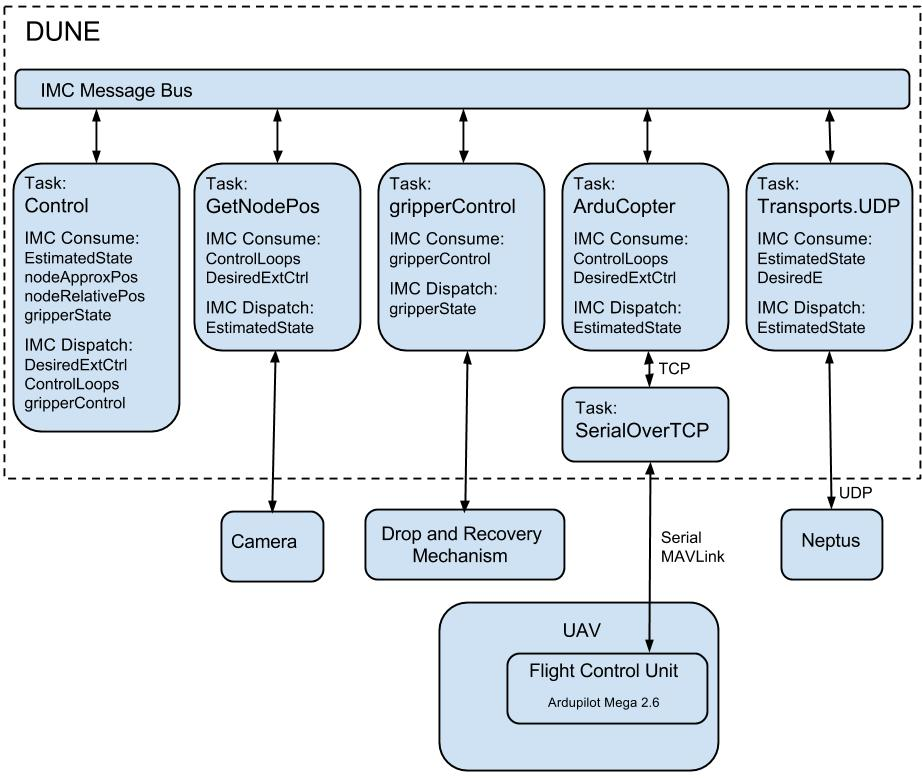
\includegraphics[width = 12cm]{fig/SW.jpg}
\caption{Software structure}
\label{SW}
\end{figure}
\subsubsection*{getNodePos}
This task uses color recognition to track the sensor node according to the procedure described in section \ref{node}. It uses the camera in combination with attitude data from the APM and sonar measurements to calculate the position of the sensor node relative to the UAV. Also the heading of the mount of the sensor node is calculated. This information and a parameter telling whether the sensor node is spotted by the camera or not is put on the IMC-bus in the nodeRelativePos message.
\subsubsection*{gripperControl}
The gripper control task consumes gripperControl messages from the IMC-bus and controls the gripper and gripperplatform according to the received commands. The gripper is controlled by setting a gripper enable and a gripper position bit on the PandaBards GPIO port. The position bit is high for open position and low or closed position. the gripperplatform is controlled by a motor which lowers and raises the platform. The motor is controlled by setting an enable bit and a direction bit on the PandaBoards GPIO port. Signals from the LED-sensor is read from the GPIO port to be able to see when the gripperplatform is in the desired position (either lowered or raised). After executing the commands it dispatches a gripperState message to the IMC-bus containing the positions of the gripper and gripperplatform.
\subsubsection*{ArduCopter}
The ArduCopter task is a result of work done by the Hexacopter group at AMOS. This task plays the role of a bridge between the APM and DUNE. ArduCopter sets up which messages that should be received from the APM and sends control messages to the APM.
\subsubsection*{Transports.UDP}
The Transports.UDP task consumes messages from the IMC bus and sends them by the use of UDP. This is used as an interface between DUNE and Neptus.
\subsubsection*{Control}
The control task is the main task in this control structure. It operates with a state variable to be able to take actions based on the phase of the mission. The different states are UNDEF, Initial searc, approching node, secondary search and node picket up. The system starts up in the UNDEF state and leaves it when it receives attitude data from the APM (via the IMC bus). Then the state switches to initial search and the UAV is guided to the approximate position of the sensor node which is given in the nodeApproxPos IMC message (this is for the time being defined by the ini file, further development will be to integrate this into Neptus). The UAV is guided towards the sensor node using the position controller described in Section \ref{pos}, the error in position is calculated by the use of  the haversine formula*. The camera is constantly searching for the sensor node while flying towards the approximate node position. When the camera finds the node the state will change to Approching node, the gripperplatform will be lowered and the gripper will be opened. In the Approaching node state the nodeRelativePos measurements will be used as feedback to the position controller. This means that the UAV will be positioned straight above the sensor node. When sufficiently close to the position straight above the sensor node will the UAV start to descend upon the sensor node. When the node is reachable to the gripper will the gripper close. If the gripper catches the node will the state change to Node picked up and the AUV will return and the gripperplatform will be raised. If while descending down upon the sensor node the camera looses sight of the sensor node, the state will change to Secondary search and the UAV will try to get back to the position of the sensor node to spot it again.